\documentclass[a4paper]{article}

\usepackage{amsmath}
\usepackage[english]{babel}
\usepackage[babel=true]{microtype}
\usepackage{wrapfig}
\usepackage{url}
\usepackage{mathrsfs} 
\usepackage[absolute]{textpos}
\usepackage{graphicx}
\usepackage{geometry}
\geometry{a4paper,left=40mm,right=30mm, top=3cm, bottom=3cm} 
\usepackage{subcaption}
\usepackage{float}

\newcommand{\Fermi}{\textit{Fermi} }

\begin{document}


\begin{figure}
	\makebox[\linewidth][c]{%
	\begin{subfigure}[b]{.5\textwidth}
		\centering
		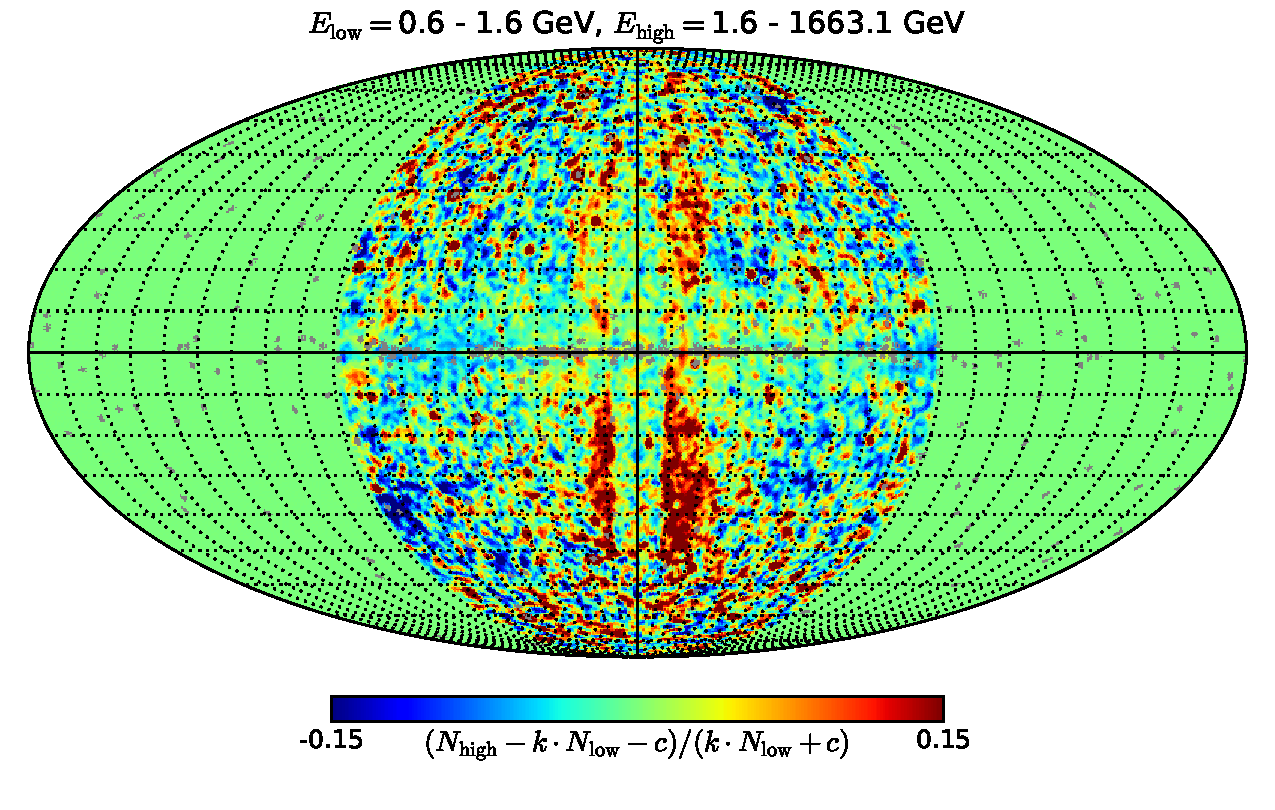
\includegraphics[width=.95\textwidth]{FitE_mollweide_at_0-1_to_1-1663_sym.pdf}
	\end{subfigure}%
	\begin{subfigure}[b]{.5\textwidth}
		\centering
		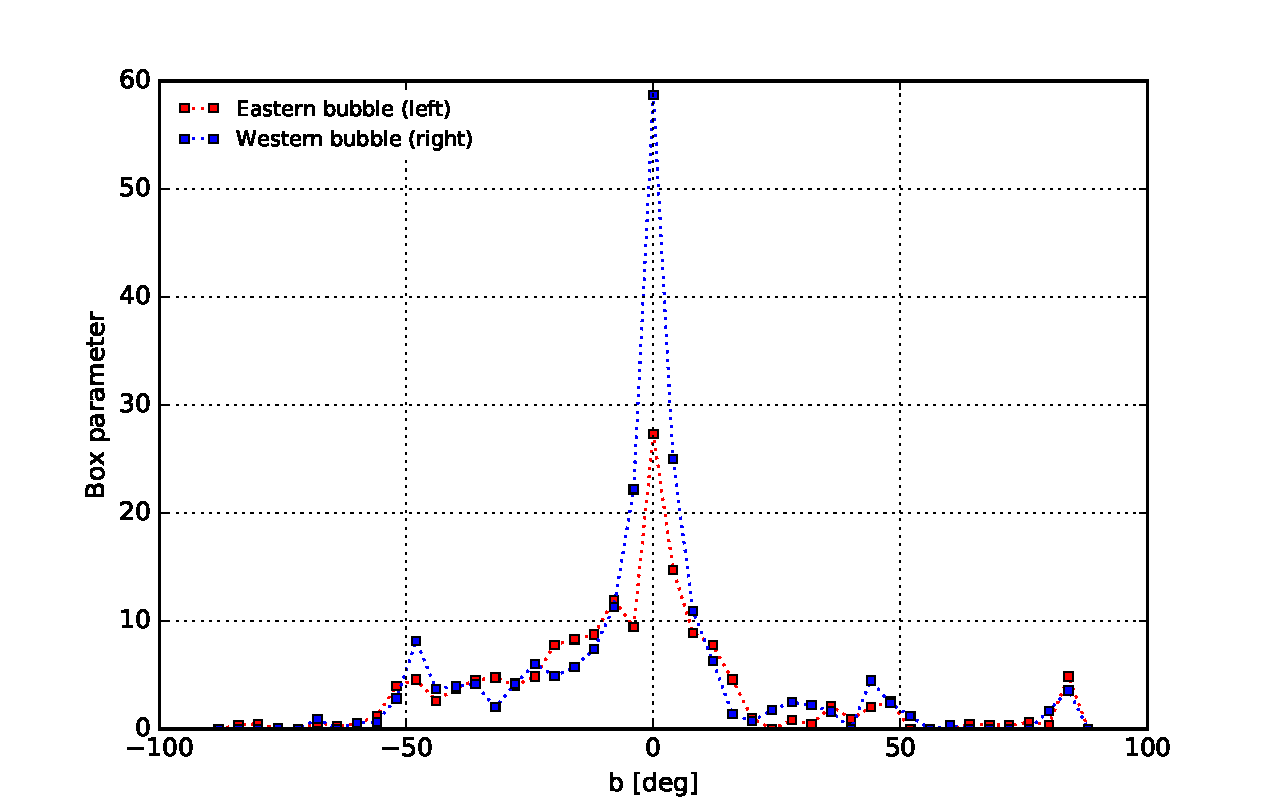
\includegraphics[width=.95\textwidth]{FitE_boxprof_at_0-1_to_1-1663_sym.pdf}
	\end{subfigure}
	%\vspace*{-3cm}
	}\\
	\makebox[\linewidth][c]{%
	\vspace*{-3cm}
	\begin{subfigure}[b]{.5\textwidth}
		\centering
		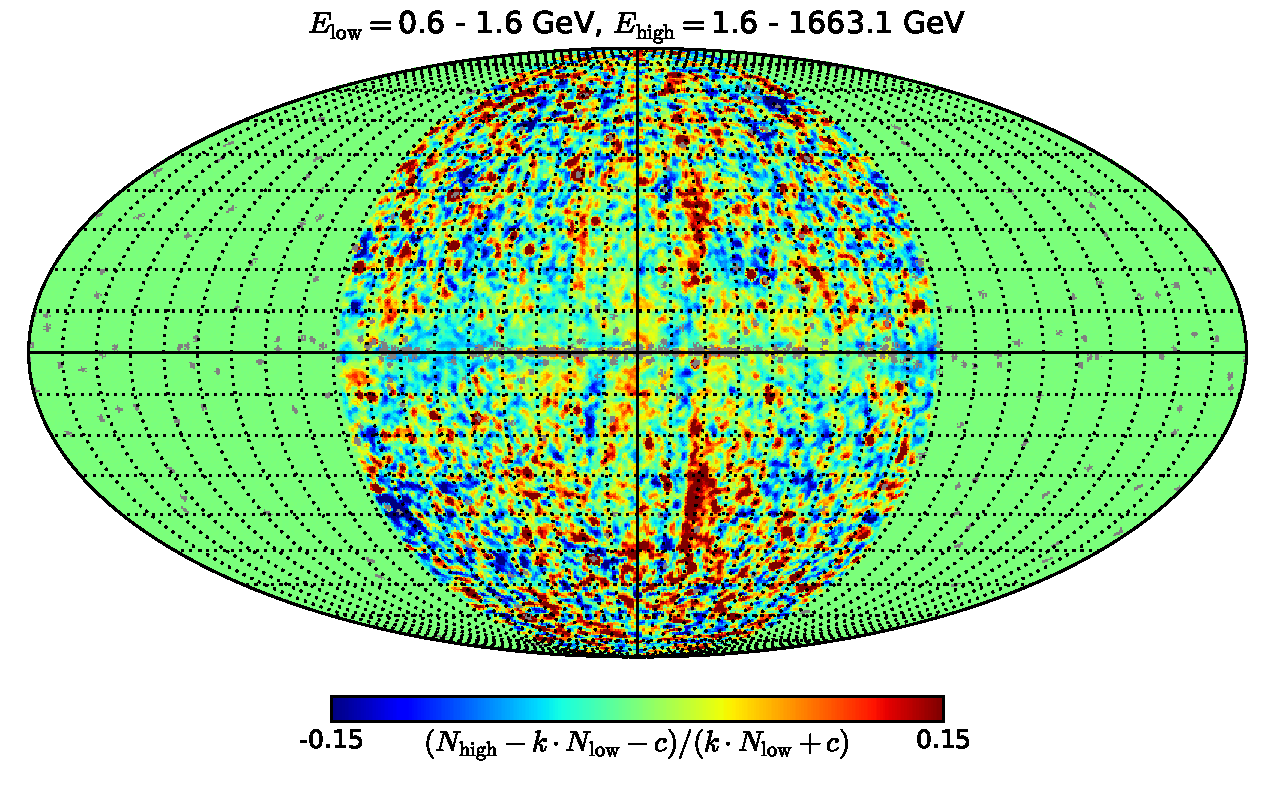
\includegraphics[width=.95\textwidth]{FitE_mollweide_at_0-1_to_1-1663_16sym.pdf}
	\end{subfigure}%
	\begin{subfigure}[b]{.5\textwidth}
		\centering
		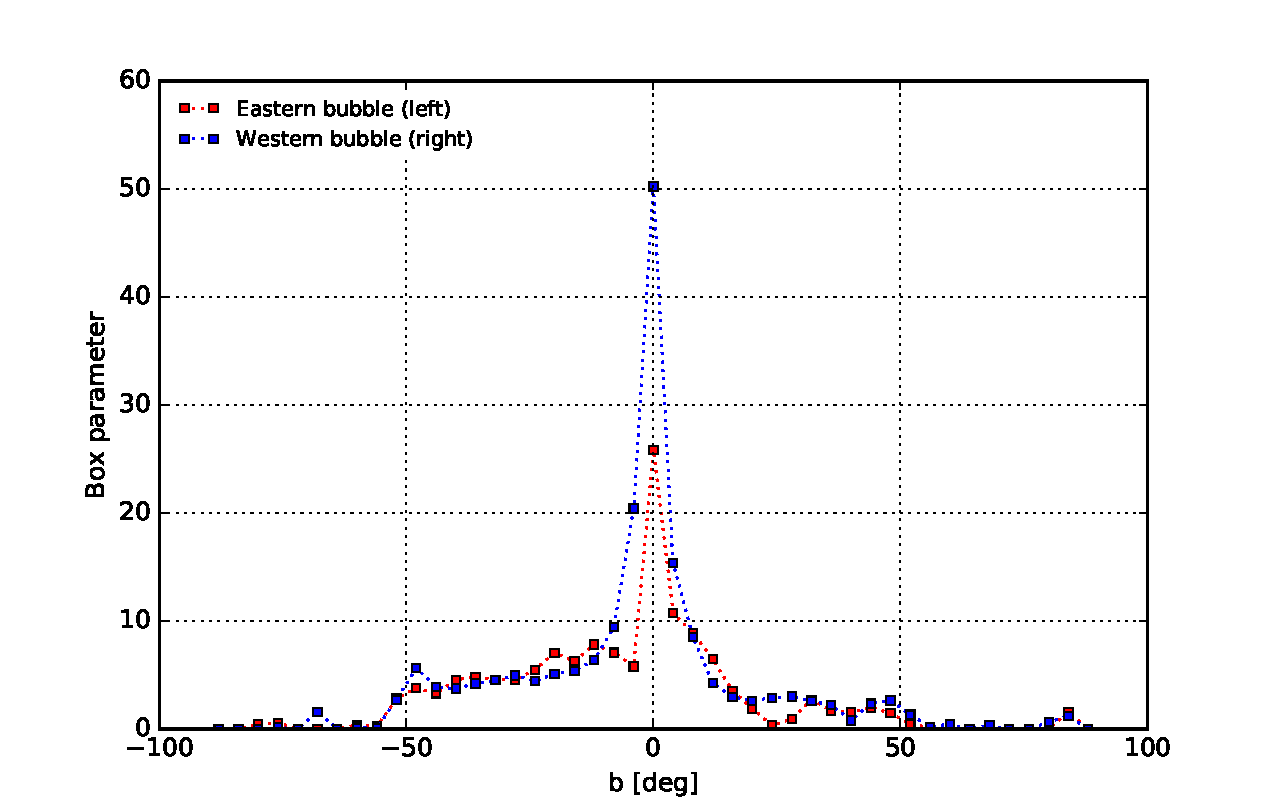
\includegraphics[width=.95\textwidth]{FitE_boxprof_at_0-1_to_1-1663_16sym.pdf}
	\end{subfigure}%
	}\\
\caption{Residual of low-energy data model with rectangles in Mollweide projection (left) and corresponding latitude profile of the box parameter (right). The box parameter is the fitting parameter of the rectangle. The rectangles are $4^\circ$ in latitude and $10^\circ$ (top row) or $16^\circ$ in longitude (bottom row). The rectangles west and east have been fitted independently. Point sources have been masked with the $0.5^\circ$ mask and the mask has been (point-)symmetrized (w.r.t. the GC). The high-energy data has been smoothed with a Gaussian of $0.5^\circ$ FWHM to compensate for the worse resolution at low energies. Only data with $|\ell| < 90^\circ$ is taken into account.}
\label{boxes_fit}
\end{figure}



\end{document}
